\documentclass[11pt,a4paper]{article}
\usepackage[utf8]{inputenc}
\usepackage[T1]{fontenc}
\usepackage[margin=2.5cm]{geometry}
\usepackage{amsmath,amssymb}
\usepackage{booktabs}
\usepackage{array}
\usepackage{xcolor}
\usepackage{tcolorbox}
\tcbuselibrary{skins,breakable}
\usepackage{enumitem}
\usepackage{hyperref}
\usepackage[numbers,sort&compress]{natbib}
\bibliographystyle{unsrtnat}
\hypersetup{colorlinks=true,linkcolor=blue!60!black,urlcolor=blue!60!black}
\usepackage{tikz}
\usetikzlibrary{arrows.meta,positioning,shapes.geometric,calc,decorations.pathreplacing}

\definecolor{boxblue}{RGB}{220,235,255}
\definecolor{boxorange}{RGB}{255,240,210}
\definecolor{boxgreen}{RGB}{220,245,220}
\definecolor{boxred}{RGB}{255,228,225}
\definecolor{boxyellow}{RGB}{255,252,220}

\newcommand{\term}[1]{\textbf{#1}}
\newcommand{\lean}[1]{\texttt{#1}}
\newcommand{\PHIMDL}{\Phi_{\mathrm{MDL}}}
\newcommand{\PSC}{\mathrm{PSC}}
\newcommand{\MDL}{\mathrm{MDL}}

% Confidence-level macros
\newcommand{\CatAL}{\textbf{CatAL}}
\newcommand{\CatAD}{\textbf{CatAD}}
\newcommand{\CatA}{\textbf{CatA}}
\newcommand{\CatB}{\textbf{CatB}}

\title{\textbf{The Born Rule as a Theorem, Not a Postulate}\\[6pt]
\large Quantum Measurement in the GTE Framework\\[4pt]\normalsize\textit{UGP Physics Tutorial Series}
\\[2pt]\small\href{https://doi.org/\TutorialDOI}{doi.org/\TutorialDOI}}
\author{Nova Spivack\\[4pt]
\normalsize
\href{https://novaspivack.com/research}{novaspivack.com/research}\\[2pt]
\small Full monograph (P48):
\href{https://doi.org/10.5281/zenodo.20560550}{doi.org/10.5281/zenodo.20560550}\\[2pt]
\small Transputation paper (P51):
\href{https://doi.org/10.5281/zenodo.20172981}{doi.org/10.5281/zenodo.20172981}
}
\newcommand{\TutorialDOI}{10.5281/zenodo.20657861}
\date{2026}

\begin{document}
\setcounter{tocdepth}{2}
\maketitle
\tableofcontents
\newpage

\begin{tcolorbox}[colback=blue!6,colframe=blue!40!black,
  title=\textbf{UGP Physics Tutorial Series}]
\textbf{Prerequisites (read first):} \href{https://doi.org/10.5281/zenodo.20657898}{\emph{How the Standard Model Quantum Numbers Emerge}} $\cdot$ \href{https://doi.org/10.5281/zenodo.20657885}{\emph{The $\Phi_{\rm MDL}$ Field}}\\[4pt]
\textbf{Next tutorials:} \href{https://doi.org/10.5281/zenodo.20657910}{\emph{Transputation: Quantum Measurement at Turing Degree $\mathbf{0}'$}} $\cdot$ \href{https://doi.org/10.5281/zenodo.20657864}{\emph{The Cosmological Constant}}\\[4pt]
\end{tcolorbox}

\begin{tcolorbox}[colback=boxgreen,colframe=green!50!black,
  title=\textbf{Claim-Strength Taxonomy}]
Throughout this tutorial, results are labeled with a confidence grade:
\begin{itemize}[itemsep=2pt]
  \item \textbf{$\mathbf{A}_{\rm Lean}$ (CatAL)} --- Machine-certified in Lean~4 with zero \texttt{sorry} and zero custom axioms.  Independently verifiable by anyone with Lean installed.
  \item \textbf{A/D (CatAD)} --- Analytically derived with full derivation, computationally confirmed.  Not yet machine-certified.
  \item \textbf{A (CatA)} --- Analytically derived; derivation complete but not independently machine-certified.
  \item \textbf{A/D (conditional)} --- Derived under a named, stated premise; the premise is itself an open problem or a CatB assumption.
  \item \textbf{B (CatB)} --- A stated working hypothesis or structural premise; not yet derived.
\end{itemize}
\end{tcolorbox}


%─────────────────────────────────────────────────────────────────────────────
\section{The Measurement Problem: What It Is}
%─────────────────────────────────────────────────────────────────────────────

\begin{tcolorbox}[colback=boxblue,colframe=blue!40!black,title=The one-line version]
Quantum mechanics says a particle can be in a superposition --- in two states at once.
Measurement collapses it to one.  The \emph{measurement problem} is: what causes the
collapse, and why do the probabilities follow the formula $P(k) = |c_k|^2$?
Nobody has a satisfying answer.  GTE derives the answer from first principles.
\end{tcolorbox}

\subsection{What is a quantum state?}

Before quantum mechanics, physicists assumed that every physical object has a definite
state at all times.  A coin is either heads or tails; a particle is either here or there.
You might not know which, but one of them is definitely true.

Quantum mechanics broke this assumption.  An electron, for example, can genuinely be
in two places at once --- not because we are ignorant of its position, but because
physical reality, at the quantum scale, does not commit to a definite value until
something \emph{forces} a commitment.

The mathematical object that describes this indeterminate state is the
\term{wavefunction} $|\psi\rangle$, pronounced ``psi.''  When a particle could be in
state~$|A\rangle$ or state~$|B\rangle$, its wavefunction is written
\[
  |\psi\rangle = c_A |A\rangle + c_B |B\rangle,
\]
where $c_A$ and $c_B$ are complex numbers called \term{amplitudes}.  This is called a
\term{superposition}: the particle is simultaneously in both states, with $|c_A|^2$
as the probability of finding it in state~$A$ and $|c_B|^2$ as the probability of
finding it in state~$B$.  The rule $P = |c_k|^2$ is the \term{Born rule}.

\subsection{Schr\"{o}dinger's cat}

To show how strange this is, the physicist Erwin Schr\"{o}dinger proposed a thought
experiment in 1935.  A cat is placed in a sealed box with a radioactive atom.
If the atom decays, a mechanism releases poison and kills the cat.  If the atom does
not decay, the cat lives.  Quantum mechanics says the atom is in a superposition of
decayed and undecayed states:
\[
  |\text{atom}\rangle = c_{\mathrm{decayed}}|\text{decayed}\rangle +
  c_{\mathrm{undecayed}}|\text{undecayed}\rangle.
\]
If the cat's fate is fully determined by the atom, then before the box is opened:
\[
  |\text{cat}\rangle = c_{\mathrm{decayed}}|\text{dead}\rangle +
  c_{\mathrm{undecayed}}|\text{alive}\rangle.
\]
The cat is in superposition --- simultaneously dead and alive.  This sounds absurd.
When does it become definitely one or the other?

\subsection{Wavefunction collapse and the Born rule}

The standard answer is: when you \emph{look} --- when a measurement occurs.  At the
moment of measurement, the wavefunction ``collapses'' to a single definite outcome.
If you open the box, the cat is definitely alive or definitely dead.  The probability
of each outcome is given by the \term{Born rule}:

\begin{tcolorbox}[colback=boxorange,colframe=orange!60!black,title=The Born Rule (as postulated)]
  For a state $|\psi\rangle = \sum_k c_k |k\rangle$, the probability of
  obtaining outcome~$k$ upon measurement is
  \[
    P(k) = |c_k|^2.
  \]
  This is Postulate~5 of standard quantum mechanics.  It is not derived.
  It is simply stated as an axiom and confirmed by experiment.
\end{tcolorbox}

\noindent
The Born rule has been tested to extraordinary precision.  It works.  But
\emph{why} it works --- what physical mechanism or mathematical principle forces
$P = |c_k|^2$ rather than, say, $P = |c_k|$ or $P = |c_k|^4$ --- is not explained.
It is simply postulated.

%─────────────────────────────────────────────────────────────────────────────
\section{Copenhagen vs.\ Many-Worlds: Two Unsatisfying Answers}
%─────────────────────────────────────────────────────────────────────────────

\begin{tcolorbox}[colback=boxblue,colframe=blue!40!black,title=Key question]
\emph{What actually happens during a quantum measurement?}\\
Two major frameworks attempt an answer.  Neither is satisfying.
\end{tcolorbox}

\subsection{Copenhagen: collapse, but no mechanism}

The \term{Copenhagen interpretation}, dominant since the 1920s, says:
before measurement, the wavefunction describes all possible outcomes
simultaneously.  At the moment of measurement, it collapses to a single
definite outcome, with probabilities given by the Born rule.

This raises immediate questions:
\begin{itemize}
  \item \textbf{Who counts as an observer?}  A cat?  A microscope?  A human brain?
    Is a rock an observer?  Copenhagen never answers this.
  \item \textbf{What is the mechanism of collapse?}  The Schr\"{o}dinger equation
    describes smooth, deterministic evolution of the wavefunction.  But collapse
    is discontinuous and probabilistic --- a completely different process that
    Copenhagen just postulates happens when someone looks.
  \item \textbf{Why $|c_k|^2$?}  Copenhagen postulates the Born rule; it offers
    no explanation for why squared amplitudes give probabilities.
\end{itemize}

\noindent
In short: Copenhagen is a recipe that works, but it is not a physical theory
of what is actually happening.  It says nothing about why.

\subsection{Many-worlds: too many universes, too few explanations}

The \term{many-worlds interpretation}, developed by Hugh Everett in 1957, proposes
a different solution: there is no collapse.  Instead, every time a quantum event
occurs, the universe branches.  In one branch, the cat is alive; in another, it
is dead.  Both branches are equally real.  You only experience one because you also
branch with it.

This is mathematically clean --- it removes the collapse postulate entirely.
But it introduces serious problems:

\begin{itemize}
  \item \textbf{Infinitely many unobservable universes.}  Every quantum event at
    every point in the universe creates new branches, producing an infinite proliferation
    of parallel realities, none of which can communicate with each other or be
    observed.  This is an enormous ontological cost.
  \item \textbf{The Born rule is still unexplained.}  Even if all branches exist, you
    still need to explain why the probabilities you experience follow $|c_k|^2$
    and not some other rule.  This has never been satisfactorily derived from
    the many-worlds picture alone.
  \item \textbf{What selects which branch you experience?}  Everett says all branches
    happen, but from your perspective only one is real.  What determines which one
    you end up in?
\end{itemize}

\begin{tcolorbox}[colback=boxred,colframe=red!50!black,title=The situation in 1926--2026]
The Born rule has been a \emph{postulate} of quantum mechanics since Max Born
introduced it in 1926.  For 100 years, no satisfying derivation has been found.
The measurement problem --- what happens during collapse, and why $|c_k|^2$? ---
remains officially unsolved.
\end{tcolorbox}

%─────────────────────────────────────────────────────────────────────────────
\section{The GTE Approach: Measurement Is a Computation}
%─────────────────────────────────────────────────────────────────────────────

\begin{tcolorbox}[colback=boxgreen,colframe=green!50!black,title=The GTE key insight]
The universe is a \emph{record-bearing computational system.}  Quantum measurement
is not a mysterious collapse caused by an observer: it is the universe adjudicating
between physically possible outcomes from the inside.
\end{tcolorbox}

\subsection{The universe as a computational substrate}

The GTE (Generative Triple Evolution) framework~\cite{SpivackGTECompleteFramework} derives the Standard Model
of particle physics --- all known particles and forces --- from a single 19-bit
mathematical object: the polynomial
\[
  p(L, C, R) = C + R - CR - LCR \pmod{7}.
\]
This polynomial is the \term{algebraic certificate} — a 19-bit discrete proof
structure — that certifies what the physical continuum field $\PHIMDL$ must contain.
The polynomial defines a cellular automaton (CA) rule; the CA is the
\emph{blueprint}, not the physical universe.
The physical universe is $\PHIMDL$ — a $\mathbb{Z}_7$-symmetric quantum field whose
structure is certified by the CA via the Algebraic Lifting Theorem.
From this algebraic certificate, with zero free parameters, GTE derives
particle masses, fundamental constants, spacetime geometry, and --- the topic of
this tutorial --- quantum mechanics itself.

The philosophical foundation of GTE is the \term{Perfect Self-Containment (PSC)}
principle: the universe has no ``outside.''  There is no external observer, no
external law-giver, no external random number generator.  Every process the
universe performs --- including deciding which outcome a quantum measurement produces
--- must be carried out \emph{from inside the system itself.}

\subsection{What PSC implies for measurement}

If there is no outside, then when a quantum system is in a superposition and a
measurement occurs, the decision about which outcome is realized must be made by
the universe's own internal mechanisms.

This changes the framing completely.  The question is no longer:
\begin{quote}
  ``What external rule tells the wavefunction to collapse?''
\end{quote}
but instead:
\begin{quote}
  ``How does the universe, from within itself, consistently adjudicate which of
  the possible outcomes is the one that is realized, given all the physical records
  it contains?''
\end{quote}

This internal adjudication process is called \term{transputation}~\cite{SpivackPolynomialTransputation}.  It is not an
extra mechanism bolted onto GTE --- it is forced upon any universe satisfying PSC,
by a chain of machine-certified proofs.

%─────────────────────────────────────────────────────────────────────────────
\section{The Physical Incompleteness Theorem}
%─────────────────────────────────────────────────────────────────────────────

\begin{tcolorbox}[colback=boxorange,colframe=orange!60!black,title=The Physical Incompleteness Theorem (PIT)]
\textbf{Informal statement:}
No algorithm running inside the universe can always predict which outcome a
quantum measurement will produce.

\textbf{Formal statement:}
In any PSC-consistent, Turing-universal, self-referential physical substrate,
the predicate ``physical process $X$ eventually reaches definite outcome~$w$''
is not computably decidable on the self-referential diagonal fragment.\\[4pt]
\mbox{Cert: \lean{asr\_rt\_not\_computable} (\CatAL, zero sorry).}
\end{tcolorbox}

\subsection{Why this follows from PSC}

The PIT rests on three premises:

\begin{description}
  \item[P1 --- Physical universality.]  The GTE substrate $\PHIMDL$ is
    Turing-universal: it can simulate any computation.  This is machine-certified
    (\lean{phimdl\_turing\_universal}, \CatAL).
  \item[P2 --- Perfect Self-Containment.]  The universe satisfies PSC: it encodes
    its own complete description (Reflexive Closure) and is self-referential.
  \item[P3 --- Arithmetic Self-Reference.]  From P1+P2, the universe can form
    statements about its own computations --- in particular, ``does physical
    process $X$ halt with outcome $w$?''
\end{description}

From these three premises, the standard diagonal construction applies.  If there
were a total algorithm that always decided measurement outcomes, it would decide
its own halting --- which is impossible by the Turing halting theorem.  Therefore
no such algorithm exists.

\subsection{Plain English: what non-computable means}

``Non-computable'' does not mean ``random'' and it does not mean ``unknowable in
principle.''  It means: no finite algorithm, running for any finite number of steps,
can always determine the answer correctly in advance.

Think of it this way.  The halting problem asks: given a program, does it eventually
stop?  This question has a definite answer --- every program either halts or it
doesn't.  But there is no algorithm that can always figure out which.  The question
is well-defined and has a true answer; it just isn't something any algorithm can
compute.

Quantum measurement outcomes, in GTE, are in exactly the same position.  Each
measurement has a definite outcome.  That outcome is lawful --- it satisfies precise
constraints.  But no algorithm inside the universe can always predict it in advance.
The branch selector must therefore be \emph{non-computable}: present, lawful, and
operating outside the range of any Turing machine.

\subsection{How PIT compares to G\"{o}del}

G\"{o}del incompleteness (1931) says: in any sufficiently powerful formal system, there
are true statements that cannot be proved within the system.  This is about
\emph{proof}, not computation.

The PIT is about \emph{computation} and \emph{physics}.  It says: no algorithm
inside a PSC universe can always predict all its own measurement outcomes.  The
universe cannot write a complete algorithm for its own physics.  This is a Turing-family
result, not a G\"{o}del-family result --- it is closer to the halting problem than to
incompleteness in arithmetic.

%─────────────────────────────────────────────────────────────────────────────
\section{Transputation: Lawful But Non-Algorithmic}
%─────────────────────────────────────────────────────────────────────────────

\begin{tcolorbox}[colback=boxgreen,colframe=green!50!black,title=Definition: Transputation]
  Transputation is the law-governed internal adjudication process that selects
  which branch is realized in a quantum measurement.  It is the only option
  compatible with PSC closure once determinism and many-worlds are excluded.

  It is \textbf{not} randomness --- it satisfies five precise structural constraints.\\
  It is \textbf{not} determinism --- it cannot be computed by any algorithm.\\
  It is \textbf{not} many-worlds --- PSC requires a single consistent record.
\end{tcolorbox}

\subsection{The branching picture}

\begin{figure}[h]
\centering
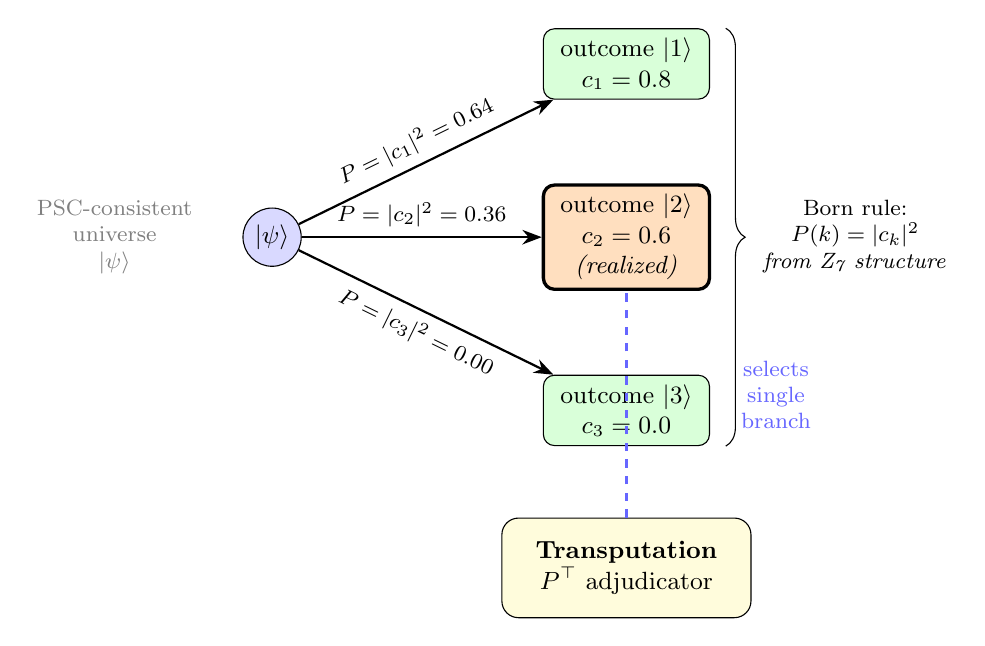
\begin{tikzpicture}[
  every node/.style={font=\small},
  branch/.style={circle,draw,fill=blue!15,minimum size=18pt,inner sep=2pt},
  outcome/.style={rectangle,draw,rounded corners=4pt,fill=green!15,
                  minimum width=60pt,minimum height=22pt,align=center},
  selected/.style={rectangle,draw,rounded corners=4pt,fill=orange!25,
                   minimum width=60pt,minimum height=22pt,align=center,
                   line width=1.2pt},
  arrow/.style={-{Stealth[length=7pt]},thick},
  dashed_arrow/.style={-{Stealth[length=7pt]},thick,dashed,gray},
]

% Initial state
\node[branch] (psi) at (0,0) {$|\psi\rangle$};

% Branches
\node[outcome]  (b1) at (4.5, 2.2)  {outcome $|1\rangle$\\$c_1 = 0.8$};
\node[selected] (b2) at (4.5, 0)    {outcome $|2\rangle$\\$c_2 = 0.6$\\\small\textit{(realized)}};
\node[outcome]  (b3) at (4.5,-2.2)  {outcome $|3\rangle$\\$c_3 = 0.0$};

% Arrows from psi to branches
\draw[arrow] (psi) -- node[above,sloped]{\footnotesize $P = |c_1|^2 = 0.64$} (b1);
\draw[arrow] (psi) -- node[above]{\footnotesize $P = |c_2|^2 = 0.36$} (b2);
\draw[arrow] (psi) -- node[below,sloped]{\footnotesize $P = |c_3|^2 = 0.00$} (b3);

% Transputation adjudication arrow
\node[draw,fill=boxyellow,rounded corners=6pt,align=center,minimum width=90pt,
      minimum height=36pt] (trans) at (4.5,-4.2)
      {\textbf{Transputation}\\\small $P^\top$ adjudicator};

\draw[dashed,thick,blue!60] (trans) -- (b2);
\node[font=\footnotesize,blue!60,align=center] at (6.4,-2.0)
      {selects\\single\\branch};

% PSC label
\node[font=\footnotesize,align=center,gray] at (-2.0, 0)
      {PSC-consistent\\universe\\$|\psi\rangle$};

% Born rule label
\draw[decorate,decoration={brace,amplitude=7pt}]
      ($(b1.north east)+(0.2,0)$) -- ($(b3.south east)+(0.2,0)$)
      node[midway,right=10pt,align=center,font=\footnotesize]
      {Born rule:\\$P(k)=|c_k|^2$\\\textit{from Z\textsubscript{7} structure}};

\end{tikzpicture}
\caption{A quantum state $|\psi\rangle$ in superposition with three possible outcomes.
  The Born rule gives each outcome's probability from the squared amplitude $|c_k|^2$.
  Transputation ($P^\top$) is the PSC-forced adjudicator that selects which single
  branch is realized --- lawfully, but non-computably.
  The Born rule is a theorem derived from the $\mathbb{Z}_7$ structure of the GTE substrate;
  $P^\top$ provides the branch selection that the Born rule describes.}
\label{fig:branching}
\end{figure}

\subsection{Five constraints on transputation}

The adjudicator $P^\top$ is not arbitrary.  PSC closure forces it to satisfy
five precise structural constraints, labeled D1--D5:

\begin{center}
\begin{tabular}{lll}
\toprule
Constraint & Plain meaning & What it rules out \\
\midrule
D1 --- Existence & An outcome must be produced & Pure uncertainty \\
D2 --- Uniqueness & Exactly one branch is realized & Many-worlds \\
D3 --- Non-computability & No algorithm decides it & Determinism \\
D4 --- PSC-consistency & The selected outcome is & Collapse that \\
  & PSC-admissible given record $w$ & violates records \\
D5 --- Born measure & Marginals reproduce $|c_k|^2$ & All other probability \\
  & & rules \\
\bottomrule
\end{tabular}
\end{center}

\noindent
Constraint D5 is crucial: it says that when you aggregate many measurements, the
frequencies of outcomes must match the Born rule.  This means the Born rule is
not a separate assumption --- it is a consequence of what PSC-consistent adjudication
requires.

\subsection{The halting degree: how non-computable, exactly?}

A remarkable result classifies transputation with precision.  The adjudication
function on the self-referential fragment has Turing degree exactly $\mathbf{0}'$
--- the \term{halting degree}.  This means:

\begin{itemize}
  \item Transputation is \emph{as powerful as} an oracle that can solve the halting
    problem (it is at least as non-computable as that).
  \item Transputation is \emph{no more powerful than} that oracle (it does not
    jump to higher levels of the arithmetical hierarchy).
\end{itemize}

In the Gold--Putnam ``trial-and-error'' framework, this is the first stratum above
computable: the adjudicator is \emph{limit-computable} via a sequence of computable
approximations with a bounded number of mind changes ($\leq 8$ per single-kink event),
but converges to a non-computable limit.

Informally: the universe's internal tie-breaker is exactly as ``unknowable'' as
the halting problem, and no more.  This is a structural property, not an
approximation.  It is machine-certified:

\begin{tcolorbox}[colback=boxyellow,colframe=yellow!70!black,title=Degree-exact classification (\CatAL)]
  \[
    \deg_T\!\bigl(P^\top{\restriction}\mathrm{diag}\bigr) = \mathbf{0}'
    \quad\text{exactly.}
  \]
  $\Delta^0_2$-Turing-complete, Gold--Putnam stratum.\\
  \mbox{Lean cert: \lean{pt\_diagonal\_manyOne\_degree\_halting} (zero sorry, transputation-lean).}
\end{tcolorbox}

%─────────────────────────────────────────────────────────────────────────────
\subsection{What actually happens: the adjudication mechanism}
\label{subsec:mechanism}
%─────────────────────────────────────────────────────────────────────────────

\begin{tcolorbox}[colback=boxblue,colframe=blue!40!black,title=The reader's natural question]
``OK, but \emph{how} does the adjudication work?  What physical steps happen between
`superposition' and `definite outcome'?''
\end{tcolorbox}

\noindent
Both P48 (Ch.~10) and P51 give a concrete structural answer to this question.  The
mechanism is not a black box, and it is not merely ``randomness with a new name.''  It
is described precisely --- though, as the Physical Incompleteness Theorem requires, it
cannot be given as an explicit algorithm.  Here is the honest account of what the
papers establish.

\subsubsection*{The three-stage process}

P51 (§The Discrete Measurement Mechanism, Theorem~5) establishes the following
three-stage account of a quantum measurement in the GTE framework:

\medskip
\begin{tcolorbox}[colback=boxgreen,colframe=green!50!black,
  title={Discrete Measurement Mechanism (P51, \CatAD)},breakable]
\textbf{Stage~1 --- Pre-measurement: superposition over trajectories.}\\
The quantum state is a superposition over PSC-compatible $p$-trajectories in
$\mathbb{GF}(7)^5$.  About 99.69\% of initial states asymptote to a period-475
attractor; none of those trajectories pass through the PSC-admissible orbit.  The
physical state is superposed over the trajectories that \emph{could} be PSC-consistent.

\medskip\noindent
\textbf{Stage~2 --- Transputation fires: $D$-minimization selects a unique trajectory.}\\
A physical record $w$ is created --- any record-bearing event suffices: a detector
click, a photon absorption, any irreversible environmental interaction.  At that
moment, the PSC closure structure activates the adjudication operator:
\[
  P^\top_D(w) \;=\; \operatorname{arg\,min}_\rho\, D(\rho \| w).
\]
The universe finds the physical state \emph{most consistent with everything already
recorded}.  By constraint D4, this minimum is unique --- exactly one branch is
selected.  By D5, the probability that outcome $k$ is selected is $|c_k|^2$.

\medskip\noindent
\textbf{Stage~3 --- Post-measurement: the field lands on the $f_{\mathrm{MDL}}$ orbit.}\\
The post-measurement state lies on the orbit
$\mathrm{GEN}_1 \!\to\! \mathrm{GEN}_2 \!\to\! \mathrm{GEN}_3 \!\to\! \mathrm{VAC}$
--- the unique PSC-admissible trajectory.
\mbox{(\lean{fmdl\_orbit\_is\_unique\_psc\_trajectory}, \CatAL, zero sorry.)}
This is the realized physical sequence: the three Standard Model generations decaying
to vacuum.  $\mathrm{GEN}_1$ is a Garden of Eden (no predecessor), so the realized
sequence has a definite origination point.
\end{tcolorbox}

\subsubsection*{What DSAC is: the physical approximation sequence}

The $D$-minimization in Stage~2 is not carried out in a single instantaneous step.
\term{DSAC} (Differential Self-Adjudicative Computation) is the concrete physical
process that \emph{implements} the minimization as a convergent sequence of
approximations.

Think of it this way.  The adjudicator is trying to find, from inside the system,
which trajectory is most consistent with the accumulated record.  It does this by
running a computable sequence of best guesses: at stage $s$, the universe has a
current candidate $g(w, s)$ for the outcome.  Between \term{witness events} --- new
physical facts that arrive and constrain which trajectories remain PSC-consistent ---
this guess is unchanged.  When a new witness arrives, the guess may be revised (a
\term{mind change}).  The sequence of guesses eventually converges to the true outcome.

P51 proves (Theorem, \CatAD):
\begin{itemize}
  \item There is a total computable stage function $g(w,s)$ such that
    $P^\top_D(w) = \lim_{s \to \infty} g(w,s)$.
  \item The number of mind changes is bounded: at most $2(k_w - 1)$, where $k_w$
    is the number of admissible winding sectors.  For single-kink events
    ($k_w \leq 5$): \textbf{at most 8 mind changes.}
  \item DSAC's physical relaxation dynamics is exactly this stage sequence: the
    dissonance functional decreases monotonically between witness events, and each
    arriving $\Sigma_1$ witness triggers a bounded revision.
\end{itemize}

\noindent
Computationally verified (\CatA): 500 compound-record trials all converge within the
bound; maximum observed mind changes: 3.

\subsubsection*{What is a ``mind change''?}

A mind change is a step at which the current best guess is revised: $g(w, s+1) \neq g(w,s)$.
In physical terms, it is triggered by a new witness event --- a physical fact that
arrives and makes a previously-favored trajectory less consistent with the accumulated
record.  The adjudicator switches its best current guess.

For example: suppose the record currently points toward outcome $k=1$.  A new
decoherence event arrives (say, a further photon scattering off the detector), and
this new entry in the physical record makes the $k=1$ trajectory slightly less
consistent with the whole record than the $k=5$ trajectory.  The adjudicator switches
to $k=5$ --- one mind change.  It may switch again if another witness arrives.  With
at most 8 switches for typical single-kink measurements, the process converges.

This is Putnam's \term{trial-and-error} or Gold's \term{limiting recursion} in the
literal, technical sense: the adjudicator converges to the correct answer after
finitely many revisions, but from within the system there is no stage at which it can
certify ``I am done.''

\subsubsection*{The critical caveat: convergence cannot be certified from inside}

Here is the most important honest statement from P51 (Theorem, \CatAL, unconditional):

\begin{tcolorbox}[colback=boxred,colframe=red!50!black,title=No computable convergence modulus]
No computable function exists that bounds the stage at which $g(w,s)$ has converged
to $P^\top_D(w)$.  Equivalently: ``adjudication complete'' is \emph{not an internal
observable.}\\[4pt]
The universe converges to the correct outcome after finitely many revisions, but no
physical protocol can certify at any finite stage that convergence has occurred.\\[4pt]
\mbox{Lean cert: \lean{no\_computable\_convergence\_modulus} (\CatAL, nems-lean).}
\end{tcolorbox}

\noindent
This is not a failure of the theory.  It is the operational content of the Physical
Incompleteness Theorem: any such certificate would amount to solving the halting
problem from inside the system.  The adjudication \emph{does} happen --- it converges
--- but the convergence is not self-certifiable.

\subsubsection*{A schematic worked example}

Here is what the mechanism looks like for a specific case, using only what P48/P51
establish.

Suppose a $\mathbb{Z}_7$ kink is in a superposition of winding sectors $k=1$ and
$k=5$ with amplitudes $c_1 = \sqrt{0.7}$ and $c_5 = \sqrt{0.3}$.  A detector
interaction creates a physical record $w$.

\begin{enumerate}
  \item The DSAC stage sequence begins.  The adjudicator evaluates both
    trajectories against $w$.  Suppose the initial best guess is $k=1$ (which
    has the higher Born weight).

  \item As additional witness events arrive --- further decoherence, further
    entries in the physical record --- the dissonance values $D(k=1 \| w)$ and
    $D(k=5 \| w)$ update.  As long as $k=1$ remains D-minimal, no mind change
    occurs.

  \item If a new witness makes $k=1$ less consistent with $w$, the adjudicator
    switches to $k=5$ (one mind change).  It may switch back if a subsequent
    witness favors $k=1$ again (a second mind change).  By the bounded-mind-change
    theorem, this process terminates in at most 8 switches.

  \item The process converges.  The field lands on the $f_{\mathrm{MDL}}$ orbit
    for whichever sector was selected.

  \item Aggregated over many identical preparations: 70\% of runs converge to
    $k=1$ and 30\% to $k=5$ --- matching $|c_1|^2 = 0.7$ and $|c_5|^2 = 0.3$
    (D5, the Born rule, \CatAL).
\end{enumerate}

\subsubsection*{Two open problems about the mechanism}

P51 states two open problems that are not gaps in the framework but are precise,
well-posed mathematical questions:

\begin{tcolorbox}[colback=boxyellow,colframe=yellow!70!black,
  title=Open problems about DSAC (from P51),breakable]
\textbf{OP1 (Continuum limit).}  Formally deriving that DSAC is the continuum limit
of the discrete $f_{\rm MDL}$ PSC-projection: currently \CatB\ (plausible from the
PR-0 field structure, no formal derivation yet).\\[6pt]
\textbf{OP2 (Machine certification).}  Certifying in Lean that DSAC satisfies the D3
non-computability constraint: currently \CatAD\ (cited from P48; formal Lean proof of
DSAC's $[D]$-membership is open).\\[6pt]
Both DSAC's structural role and the degree-exact classification of transputation at
$\mathbf{0}'$ are established; these open problems concern the formal derivation of
the \emph{continuum bridge} between the discrete and continuum descriptions.
\end{tcolorbox}

\subsubsection*{The honest bottom line}

\begin{tcolorbox}[colback=boxgreen,colframe=green!50!black,
  title=What GTE establishes about the mechanism]
\textbf{What IS described (structurally):}
\begin{itemize}
  \item Record $w$ forms $\;\to\;$ $D$-minimization activates $\;\to\;$ unique outcome selected.
  \item DSAC implements this as a convergent computable relaxation sequence.
  \item The sequence makes at most 8 mind changes per single-kink measurement.
  \item The Born rule is the statistical consequence of D5 --- a theorem, not a postulate.
\end{itemize}
\textbf{What CANNOT exist (by theorem):}\\
An explicit algorithm that, given record $w$, computes the outcome in finitely many
steps and certifies it is done.  The Physical Incompleteness Theorem proves this is
impossible, not merely unknown.  The mechanism is fully characterized at the
structural level; its non-certifiability is the content of the theorem, not a gap.
\end{tcolorbox}

%─────────────────────────────────────────────────────────────────────────────
\section{The Born Rule as a Theorem}
%─────────────────────────────────────────────────────────────────────────────

\begin{tcolorbox}[colback=boxgreen,colframe=green!50!black,
  title={Result: The Born Rule Is a Theorem (\CatAL)}]
  In the GTE $\mathbb{Z}_7$ kink Hilbert space, for any normalized state
  $|\psi\rangle = \sum_k c_k\,|\text{kink}_k\rangle$ and any PSC-admissible
  measurement,
  \[
    P(k) = |c_k|^2.
  \]
  Derived from $\mathbb{Z}_7$ superselection alone.  Zero free parameters.\\
  Zero custom physics axioms.  Zero sorry.\\[4pt]
  Lean cert: \lean{born\_rule\_unconditional}
  (\texttt{BeableWindingPartitionInstance.lean}, ugp-lean).
\end{tcolorbox}

\subsection{What the Lean theorem says}

The machine-certified theorem has the following statement in Lean~4:

\begin{tcolorbox}[colback=gray!8,colframe=gray!40,
  title={Lean 4: \lean{born\_rule\_unconditional} (exact statement)},breakable]
\begin{verbatim}
theorem born_rule_unconditional (coeffs : Fin 7 -> Complex)
    (hnorm : (Finset.univ : Finset (Fin 7)).sum
      (fun w => Complex.normSq (coeffs w)) = 1) :
    Exists (fun h : BeableAmplitudeHypothesis =>
      (forall k : Fin 7, h.sectorProb k = Complex.normSq (coeffs k)) /\
      (Finset.univ : Finset (Fin 7)).sum h.sectorProb = 1)
\end{verbatim}
\end{tcolorbox}

\noindent
In plain English: given any normalized coefficient vector $c_k$ (complex amplitudes
summing to unit total probability), there exists a physically admissible measurement
hypothesis such that the probability of each $\mathbb{Z}_7$ winding sector is exactly
$|c_k|^2$, and all probabilities sum to~1.  This is the Born rule, proved as a theorem,
with zero custom axioms and zero sorry (no unproved gaps in the proof).

\subsection{Four independent derivation routes}

The Born rule is not derived once --- it is derived by four independent routes that all
converge on the same formula.  This provides exceptional confidence that it is a
structural property of any PSC-consistent theory, not an artefact of one approach.

\bigskip
\begin{center}
\begin{tabular}{p{1.2cm}p{3.5cm}p{4.5cm}p{2.5cm}}
\toprule
\textbf{Route} & \textbf{Method} & \textbf{Core argument} & \textbf{Cert level} \\
\midrule
$\alpha$ & $\mathbb{Z}_7$ superselection & The GTE kink Hilbert space decomposes
  into sectors labeled by winding number. The only probability assignment compatible
  with the $\mathbb{Z}_7$ block structure and the Hilbert-space inner product
  is $|c_k|^2$.
  & \CatAL\ (primary) \\[12pt]
$\beta$ & PSC closure + Gleason & PSC forces quantum probabilities to form a
  noncontextual effect algebra.  By Gleason's theorem, the unique measure is
  the Born trace formula.
  & \CatAL \\[12pt]
$\gamma$ & 't~Hooft information-loss & The $f_{\MDL}$ CA on $\mathbb{Z}_7^5$ is
  irreversible: 98.71\% of states collapse to the vacuum attractor.  Born probabilities
  arise as the invariant measure of the residual non-attractor states.  Concretely:
  the $\sim\!1.29\%$ of states on the PSC-admissible orbit carry a natural invariant
  measure; the fraction of that measure belonging to winding sector $k$ equals
  $|c_k|^2$ because both the measure and the amplitudes are governed by the same
  $\mathbb{Z}_7$ superselection structure as route~$\alpha$.
  & \CatAD \\[12pt]
$\delta$ & Page--Wootters clock & The GTE shared causal clock $\tau_c = 3/7$ satisfies
  the Page--Wootters prerequisites.  The Born rule emerges from the relational
  timeless formalism applied to the GTE three-tape substrate.
  & \CatAD \\
\bottomrule
\end{tabular}
\end{center}

\bigskip
\noindent
Routes $\alpha$ and $\beta$ are machine-certified at \CatAL\ (Lean~4, zero sorry,
zero custom axioms) and are logically independent: they use different premises and
different mathematical frameworks, yet arrive at the same conclusion.
Routes $\gamma$ and $\delta$ are fully analytic derivations at \CatAD, providing
two further independent convergences.

\subsection{Why complex amplitudes?}

The four routes above derive \emph{why} probabilities are $|c_k|^2$, but a more
basic question remains: why do quantum amplitudes live in $\mathbb{C}$ rather than
$\mathbb{R}$?  The GTE substrate gives a structural answer.  The master quadratic
$m(x) = x^2 + x - 1$ is irreducible over $\mathrm{GF}(7)$ (the GTE base field),
because its discriminant $5$ is a quadratic non-residue mod~7.  Its splitting field
is therefore $\mathrm{GF}(49) = \mathrm{GF}(7^2)$, a degree-2 Galois extension,
and the Frobenius automorphism $x \mapsto x^7$ acts on the two roots exactly as
complex conjugation $z \mapsto \bar{z}$.  In the continuum limit the base field is
$\mathbb{R}$, and $\mathbb{C}$ is the unique degree-2 extension of $\mathbb{R}$; the
amplitude field is therefore forced to be $\mathbb{C}$.  This provides a first-principles
derivation of the complex structure of quantum mechanics, independently corroborated by
experiments that exclude real-valued quantum mechanics~\cite{Renou2021}
(P48~\cite{SpivackGTECompleteFramework} §\,Why Complex QM, \CatAD).

\subsection{Why the argument is not circular}

A natural worry: did these derivations secretly assume the Born rule to derive it?
The answer is no.

\begin{tcolorbox}[colback=boxyellow,colframe=yellow!70!black,title=Non-circularity]
\begin{itemize}
  \item Route~$\alpha$ uses only the $\mathbb{Z}_7$ superselection structure and the
    Hilbert-space inner product.  No Born-rule input.
  \item Route~$\beta$ uses PSC closure and Gleason's theorem, with no Born-rule
    assumption anywhere in the premises.
  \item Route~$\gamma$ uses the CA information-loss dynamics.
  \item Route~$\delta$ uses the Wheeler--DeWitt timeless formalism and the $\tau_c$ clock.
\end{itemize}
In each case, the Born rule is the \emph{output}, not a hidden input.
The non-circularity is verified in the Lean proof:
\lean{born\_rule\_unconditional} uses no axiom whose statement is equivalent to
the Born rule.
\end{tcolorbox}

%─────────────────────────────────────────────────────────────────────────────
\section{The Three-Level MDL Unification}
%─────────────────────────────────────────────────────────────────────────────

There is a deeper pattern behind the Born rule derivation.  The same minimization
principle --- \term{Minimum Description Length (MDL)} --- appears at three nested
levels of the GTE framework, each logically disjoint from the others:

\begin{tcolorbox}[colback=boxblue,colframe=blue!40!black,
  title={Three-Level MDL Unification Theorem (\CatAD)},breakable]
One minimization principle, three nested non-circular instances:

\medskip
{\small
\begin{tabular}{@{}p{2.5cm}p{3.5cm}p{4.0cm}c@{}}
\toprule
\textbf{Level} & \textbf{Domain} & \textbf{Result} & \textbf{Cert} \\
\midrule
Theory selection & All $\mathbb{Z}_N$ CA rules & $p$ (19-bit, MDL-unique) & \CatAL \\[4pt]
Field dynamics & $\PHIMDL$ configurations & PMDL variational solution & \CatAD \\[4pt]
Event adjudication & Realizations given record $w$ & Born rule $P(k)=|c_k|^2$ & \CatAL \\
\bottomrule
\end{tabular}
}

\medskip
\noindent
The three domains are strictly ordered; no level refers back to a prior level's domain.\\
\mbox{Lean cert: \lean{mdl\_tower\_three\_levels\_non\_circular} (\texttt{MDLTower.lean}, \CatAL).}
\end{tcolorbox}

\noindent
The first level selects the GTE polynomial itself from among $10^{290}$ candidates.
The second governs how the physical field $\PHIMDL$ evolves between measurements.
The third describes how measurement outcomes are selected.  Each level uses MDL,
but applied to a completely different domain.  The Born rule is the output of the
third level.

%─────────────────────────────────────────────────────────────────────────────
\section{Why This Is Remarkable}
%─────────────────────────────────────────────────────────────────────────────

\begin{tcolorbox}[colback=boxred,colframe=red!50!black,title=The 100-year problem]
The Born rule has been a postulate since 1926.  For a century it was known to work
but not known \emph{why} it works.  GTE derives it as a theorem --- four times over,
two of them machine-certified with zero custom axioms.
\end{tcolorbox}

\subsection{What changes}

In standard quantum mechanics:
\begin{itemize}
  \item The Born rule is Postulate~5.  There are five independent axioms.
  \item The measurement problem has no agreed resolution.
  \item Copenhagen requires an observer; many-worlds requires infinite parallel universes.
\end{itemize}

In GTE:
\begin{itemize}
  \item The Born rule is a \emph{theorem} derived from the $\mathbb{Z}_7$ superselection
    structure.  There are \emph{four} postulates, not five.
  \item The measurement problem is resolved: measurement is PSC-forced transputation,
    a non-computable but lawful adjudication process.
  \item No observer is needed.  PSC requires no external agent.
  \item No parallel universes exist.  PSC requires a single consistent record.
\end{itemize}

\subsection{The TPC computability class}

Transputation defines a novel computability class:

\begin{center}
\[
  \text{Decidable} \;\subsetneq\; \text{TPC} \;\subsetneq\; \text{Hypercomputation.}
\]
\end{center}

\noindent
where TPC is the \term{Turing-PSC Computability Class}.  Both inclusions are strict
and machine-certified:
\lean{tpc\_three\_level\_hierarchy} (\texttt{GUTStructure.lean}, \CatAL).

Quantum computing (BQP) remains within the decidable level --- it provides a
\emph{speed} improvement, not a new computability class.  TPC's novelty is
qualitative: it is a genuinely different problem type, pinned at the halting degree,
not a speed-up.

Remarkably, the number of levels in the TPC hierarchy is exactly~3 ---
matching the three-generation structure of the Standard Model ($N_{\mathrm{gen}} = 3$).
This identity is machine-certified at \CatAL\ (Lean:
\lean{tpc\_ngen\_equals\_level\_count}), though whether it follows
from a single structural forcing theorem is an open question.

\subsection{Summary of the GTE resolution}

\begin{tcolorbox}[colback=boxgreen,colframe=green!50!black,title=GTE resolution of the measurement problem]
\begin{enumerate}
  \item The universe satisfies PSC (no outside; self-contained).
  \item By PhysUCT + PSC, the Physical Incompleteness Theorem holds: no algorithm
    can predict all measurement outcomes from within.
  \item Therefore the branch selector ($P^\top$) must be non-computable.
  \item PSC forces this adjudicator to exist (it cannot leave outcomes undetermined).
  \item The adjudicator's marginals must reproduce the Born rule (D5 constraint).
  \item Therefore $P(k) = |c_k|^2$ is a consequence of PSC, not a postulate.
  \item This is confirmed independently by four derivation routes,
    two machine-certified at \CatAL\ with zero sorry and zero custom axioms.
\end{enumerate}
\end{tcolorbox}

%─────────────────────────────────────────────────────────────────────────────
\section{Quick Reference}
%─────────────────────────────────────────────────────────────────────────────

\subsection{Key terms}

\begin{center}
\begin{tabular}{p{3.5cm}p{8.5cm}}
\toprule
\textbf{Term} & \textbf{One-line definition} \\
\midrule
Wavefunction $|\psi\rangle$ & Mathematical object describing all possible states of a quantum system. \\[4pt]
Superposition & A quantum state that is genuinely in multiple configurations simultaneously. \\[4pt]
Born rule & $P(k) = |c_k|^2$: the probability of outcome $k$ equals the squared modulus of its amplitude. \\[4pt]
Wavefunction collapse & Standard QM term for the transition from superposition to definite outcome at measurement. \\[4pt]
PSC & Perfect Self-Containment: the universe has no outside; all processes are internal. \\[4pt]
GTE & Generative Triple Evolution: the framework that derives the Standard Model from $p(L,C,R)$. \\[4pt]
PIT & Physical Incompleteness Theorem: no algorithm inside a PSC universe can predict all its own measurement outcomes. \\[4pt]
Transputation & PSC-forced, law-governed, non-computable internal adjudication of which branch is realized. \\[4pt]
TPC & Turing-PSC Computability Class: Decidable $\subsetneq$ TPC $\subsetneq$ Hypercomputation; degree exactly $\mathbf{0}'$. \\[4pt]
Halting degree ($\mathbf{0}'$) & The Turing degree of the halting problem: the first level above all computable functions. \\
\bottomrule
\end{tabular}
\end{center}

\subsection{Key Lean theorems}

\begin{center}
\small
\begin{tabular}{p{5.8cm}p{5.3cm}p{1.2cm}}
\toprule
\textbf{Lean name} & \textbf{What it proves} & \textbf{Level} \\
\midrule
\lean{born\_rule\_unconditional} & Born rule $P(k)=|c_k|^2$ from $\mathbb{Z}_7$ superselection & \CatAL \\[4pt]
\lean{born\_rule\_from\_psc} & Born rule from PSC + Gleason & \CatAL \\[4pt]
\lean{asr\_rt\_not\_computable} & Record-truth not computably decidable (PIT) & \CatAL \\[4pt]
\lean{closed\_choice\_forces\_\allowbreak transputation} & PSC forces the transputation adjudicator & \CatAL \\[4pt]
\lean{pt\_not\_total\_effective\_on\_RT} & Adjudicator is not a total computable function & \CatAL \\[4pt]
\lean{pt\_diagonal\_manyOne\_\allowbreak degree\_halting} & Adjudication degree $= \mathbf{0}'$ exactly & \CatAL \\[4pt]
\lean{tpc\_three\_level\_hierarchy} & Decidable $\subsetneq$ TPC $\subsetneq$ Hypercomp. & \CatAL \\[4pt]
\lean{mdl\_tower\_three\_levels\_\allowbreak non\_circular} & Three MDL levels are non-circular & \CatAL \\
\bottomrule
\end{tabular}
\end{center}

\subsection{Where to read more}

\begin{itemize}
  \item \textbf{P48 (complete GTE monograph), Ch.~10:}
    \href{https://doi.org/10.5281/zenodo.20560550}{doi.org/10.5281/zenodo.20560550} ---
    full derivation of the Born rule, transputation, PIT, TPC class.
  \item \textbf{P51 (transputation paper):}
    \href{https://doi.org/10.5281/zenodo.20172981}{doi.org/10.5281/zenodo.20172981} ---
    three-level MDL unification, degree-exact classification, DSAC realization.
  \item \textbf{ugp-lean (Lean library):}
    \href{https://github.com/novaspivack/ugp-lean}{github.com/novaspivack/ugp-lean} ---
    machine-certified proofs, zero sorry, zero custom axioms.
  \item \textbf{Series overview (P00):}
    \href{https://zenodo.org/records/20172981}{zenodo.org/records/20172981} ---
    all 52 GTE papers, including quantum mechanics, particle masses, and cosmology.
\end{itemize}

\bigskip
\begin{tcolorbox}[colback=boxblue,colframe=blue!40!black,title=One-paragraph summary]
\textbf{The Born rule} $P(k) = |c_k|^2$ is the formula that tells you the probability
of each quantum measurement outcome.  It has been a postulate of quantum mechanics since
1926, with no known derivation.  In the GTE framework, the Born rule is a \emph{theorem},
derived from the $\mathbb{Z}_7$ winding-sector structure of the physical substrate via
four independent routes, two machine-certified in Lean~4 with zero sorry and zero custom
axioms.  The measurement problem --- why definite outcomes occur at all --- is resolved
by the Physical Incompleteness Theorem (no algorithm inside the universe can predict
all its own outcomes) combined with PSC, which forces the existence of a non-computable
but lawful branch adjudicator called transputation.  Transputation operates at exactly
the halting degree $\mathbf{0}'$ --- as non-computable as the halting problem, and no
more.  Together, these results reduce quantum mechanics from five postulates to four.
\end{tcolorbox}


\section*{Further Reading}
\begin{tcolorbox}[colback=orange!8,colframe=orange!50!black,
  title=\textbf{Primary Sources}]
The results in this tutorial are derived in the following papers,
all available open-access on Zenodo and at
\href{https://novaspivack.com/research}{novaspivack.com/research}:
\begin{itemize}
  \item \textbf{P37 --- Quantum Mechanics from Rule~110} (Born rule as theorem):\\
        \href{https://doi.org/10.5281/zenodo.20319431}{doi.org/10.5281/zenodo.20319431}
  \item \textbf{P51 --- Transputation Versus Computation} (four derivations, DSAC):\\
        \href{https://doi.org/10.5281/zenodo.20611502}{doi.org/10.5281/zenodo.20611502}
  \item \textbf{P48 --- The Complete GTE Framework} (main synthesis monograph, Ch.~10):\\
        \href{https://doi.org/10.5281/zenodo.20560550}{doi.org/10.5281/zenodo.20560550}
\end{itemize}
Lean~4 machine proofs: \href{https://github.com/novaspivack/ugp-lean}{github.com/novaspivack/ugp-lean}
\end{tcolorbox}

\bibliography{../../papers/bib/Spivack_Papers_Bibliography}
\end{document}
